\documentclass{standalone}

\usepackage{tikz}
\usetikzlibrary{shapes,arrows,positioning,shapes.geometric}
\usepackage{ifthen}

\setlength{\textwidth}{40cm}

\begin{document}
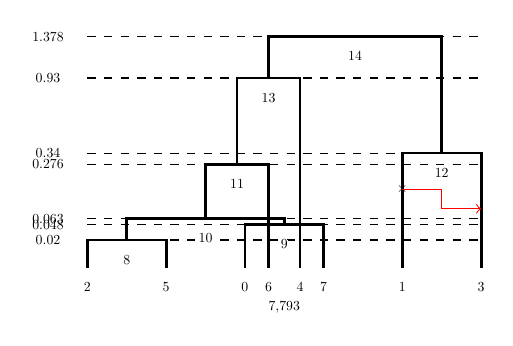
\begin{tikzpicture}

\def\hstep{.5pt}
\def\vstep{.25pt}

\def\pone{{2, 0, 8, 6, 1, 4, 12}}
\def\ptwo{{5, 7, 9, 10, 3, 11, 13}}
\def\site{7793}
\def\X{{4, 8, 0, 10, 5.4, 2, 4.6, 6, 1.0, 5.0, 3.0, 3.8, 9.0, 4.6, 6.8}}
\def\minx{0.000000}
\def\maxx{10.000000}
\def\T{{0.0, 0.0, 0.0, 0.0, 0.0, 0.0, 0.0, 0.0, 0.020048361376906708, 0.04801085544951425, 0.0625853218585976, 0.27555736060975966, 0.33999774845294395, 0.9304928979569461, 1.3783535219342424}}
\def\Tnorm{{0.0, 0.0, 0.0, 0.0, 0.0, 0.0, 0.0, 0.0, 1.4159223628754054, 2.1911379566224087, 2.5017058551835705, 5.2493557758048714, 5.830932587956612, 9.646205979331699, 11.740330156917405}}
\def\LAB{{0, 1, 2, 3, 4, 5, 6, 7, 8, 9, 10, 11, 12, 13, 14}}
\def\coloring{-1}
\def\globalindex{{0, 1, 2, 3, 4, 5, 6}}
\def\globalindiceson{-1}
\def\regrafttime{0}
\def\regrafttimenorm{3}
\def\recombinationtime{0}
\def\recombinationtimenorm{4}
\def\NL{8}
\def\NN{15}
\def\prune{1}
\def\regraft{3}

\def\prpar{-1}
\def\rgpar{-1}

\def\newnode{-1}

% Copyright (C) 2016, Kari Heine, Maria De Iorio, Alex Beskos, Ajay Jasra,
% David Balding. All rights reserved.
%
% Redistribution and use in source and binary forms, with or without
% modification, are permitted provided that the following conditions
% are met:
%
%   1. Redistributions of source code must retain the above copyright
%      notice, this list of conditions and the following disclaimer.
%
%   2. Redistributions in binary form must reproduce the above copyright
%      notice, this list of conditions and the following disclaimer in the
%      documentation and/or other materials provided with the distribution.
%
%   3. The names of its contributors may not be used to endorse or promote
%      products derived from this software without specific prior written
%      permission.
%
% THIS SOFTWARE IS PROVIDED BY THE COPYRIGHT HOLDERS AND CONTRIBUTORS
% "AS IS" AND ANY EXPRESS OR IMPLIED WARRANTIES, INCLUDING, BUT NOT
% LIMITED TO, THE IMPLIED WARRANTIES OF MERCHANTABILITY AND FITNESS FOR
% A PARTICULAR PURPOSE ARE DISCLAIMED.  IN NO EVENT SHALL THE COPYRIGHT OWNER OR
% CONTRIBUTORS BE LIABLE FOR ANY DIRECT, INDIRECT, INCIDENTAL, SPECIAL,
% EXEMPLARY, OR CONSEQUENTIAL DAMAGES (INCLUDING, BUT NOT LIMITED TO,
% PROCUREMENT OF SUBSTITUTE GOODS OR SERVICES; LOSS OF USE, DATA, OR
% PROFITS; OR BUSINESS INTERRUPTION) HOWEVER CAUSED AND ON ANY THEORY OF
% LIABILITY, WHETHER IN CONTRACT, STRICT LIABILITY, OR TORT (INCLUDING
% NEGLIGENCE OR OTHERWISE) ARISING IN ANY WAY OUT OF THE USE OF THIS
% SOFTWARE, EVEN IF ADVISED OF THE POSSIBILITY OF SUCH DAMAGE.
 
% --------------------------------------------------------------------
% --------------------------------------------------------------------
% Tree site
% --------------------------------------------------------------------
% --------------------------------------------------------------------
\pgfmathsetmacro{\xsite}{(\minx+\maxx)/2*\hstep}
\pgfmathsetmacro{\ysite}{-2*\vstep}
\pgfmathsetmacro{\sitelab}{\site}

\node[scale=.5] at (\xsite,\ysite) {\pgfmathprintnumber[fixed,precision=0]{\sitelab}};

% --------------------------------------------------------------------
% --------------------------------------------------------------------
% Draw time grid
% --------------------------------------------------------------------
% --------------------------------------------------------------------
\pgfmathsetmacro{\nb}{\NL-2}
\foreach \i in {0,...,\nb} 
{
	\pgfmathsetmacro{\y}{\Tnorm[\NL+\i]*\vstep}
	\pgfmathsetmacro{\xs}{\minx*\hstep}
	\pgfmathsetmacro{\xe}{\maxx*\hstep}
	\pgfmathsetmacro{\xt}{(\minx-1)*\hstep}
	\pgfmathsetmacro{\tlab}{\T[\NL+\i]}
	
	\draw[-,dashed] (\xs,\y) -- (\xe,\y);
	
	\node[scale=.5] at (\xt,\y) {\pgfmathprintnumber[fixed,precision=3]{\tlab}};
}

% --------------------------------------------------------------------
% --------------------------------------------------------------------
% Draw the coalescent tree
% --------------------------------------------------------------------
% --------------------------------------------------------------------
\pgfmathsetmacro{\maxit}{\NN-1}
\foreach \i in {0,...,\maxit}
{
	\pgfmathsetmacro{\x}{\X[\i]*\hstep}
	\pgfmathsetmacro{\y}{\Tnorm[\i]*\vstep}
	
	\ifthenelse{\i=\NL \OR \i>\NL}{
	
		\pgfmathsetmacro{\signL}{int(\pone[\i-\NL])}
		\pgfmathsetmacro{\signR}{int(\ptwo[\i-\NL])}
		
		
		\ifthenelse{\signL>-1 \AND \signR>-1}{
			\pgfmathsetmacro{\xl}{\X[\pone[\i-\NL]]*\hstep}
			\pgfmathsetmacro{\yl}{\Tnorm[\pone[\i-\NL]]*\vstep}
			\pgfmathsetmacro{\xr}{\X[\ptwo[\i-\NL]]*\hstep}
			\pgfmathsetmacro{\yr}{\Tnorm[\ptwo[\i-\NL]]*\vstep}
			\draw[-,line width = 1pt] (\xl,\yl) -- (\xl,\y) -- (\xr,\y) -- (\xr,\yr);		
		}{};
		
		\ifthenelse{\signL<0 \AND \signR>-1}{
			\pgfmathsetmacro{\xr}{\X[\ptwo[\i-\NL]]*\hstep}
			\pgfmathsetmacro{\yr}{\Tnorm[\ptwo[\i-\NL]]*\vstep}
			\draw[-,line width = 1pt] (\xr,\y) -- (\xr,\yr);		
		}{};
		\ifthenelse{\signL>-1 \AND \signR<0}{
			\pgfmathsetmacro{\xl}{\X[\pone[\i-\NL]]*\hstep}
			\pgfmathsetmacro{\yl}{\Tnorm[\pone[\i-\NL]]*\vstep}
			\draw[-,line width = 1pt] (\xl,\yl) -- (\xl,\y);		
		}{};
	}{};		
}

% --------------------------------------------------------------------
% --------------------------------------------------------------------
% Draw coloured nodes
% --------------------------------------------------------------------
% --------------------------------------------------------------------
\ifthenelse{\coloring>-1}{
\foreach \i in {0,...,\maxit}
{
	\pgfmathsetmacro{\x}{\X[\i]*\hstep}
	\pgfmathsetmacro{\y}{\Tnorm[\i]*\vstep}
	\pgfmathsetmacro{\clr}{\colors[\i]}
	
	\ifthenelse{\clr=2}{
	\node[draw,circle,fill=white, inner sep =0pt, minimum size = 2mm] at (\x,\y) {};
	}{
	\ifthenelse{\clr=0}{
	\node[draw,circle,fill=black, inner sep =0pt, minimum size = 2mm] at (\x,\y) {};
	}{
	\node[draw,circle,fill=gray, inner sep =0pt, minimum size = 2mm] at (\x,\y) {};
	};
	};
	
}
}{};

% --------------------------------------------------------------------
% --------------------------------------------------------------------
% Node labels
% --------------------------------------------------------------------
% --------------------------------------------------------------------
\foreach \i in {0,...,\maxit}
{	
	\pgfmathsetmacro{\x}{\X[\i]*\hstep}
	\pgfmathsetmacro{\y}{\Tnorm[\i]*\vstep-1*\vstep}
	\pgfmathsetmacro{\lab}{\LAB[\i]}	

	\node[fill=white,inner sep =0pt, scale=.5] at (\x,\y) {\pgfmathprintnumber[fixed,precision=0]{\lab}};
	
}
% --------------------------------------------------------------------
% --------------------------------------------------------------------
% Global indexing
% --------------------------------------------------------------------
% --------------------------------------------------------------------
\ifthenelse{\globalindiceson>0}{
\pgfmathsetmacro{\nbmaxit}{\NL-2}
\foreach \i in {0,...,\nbmaxit}
{	
	\pgfmathsetmacro{\x}{\X[\i+\NL]*\hstep+.5*\hstep}
	\pgfmathsetmacro{\y}{\Tnorm[\i+\NL]*\vstep+.5*\vstep}
	\pgfmathsetmacro{\glab}{\globalindex[\i]}

	\node[fill=white,inner sep =0pt, scale=.5] at (\x,\y) {\pgfmathprintnumber[fixed,precision=0]{\glab}};
	
}
}{};

% --------------------------------------------------------------------
% --------------------------------------------------------------------
% Operation
% --------------------------------------------------------------------
% --------------------------------------------------------------------
\ifthenelse{\prune>-1}{

	% operation start point
	\pgfmathsetmacro\rectimesign{int(round(\recombinationtime))}
	\ifthenelse{\rectimesign<0}{

		\pgfmathsetmacro{\xstart}{\X[\prune]*\hstep}
		\pgfmathsetmacro{\ystart}{\Tnorm[\prune]*\vstep + (\Tnorm[\prpar] - \Tnorm[\prune])/2*\vstep}

	}{

		\pgfmathsetmacro{\xstart}{\X[\prune]*\hstep}
		\pgfmathsetmacro{\ystart}{\recombinationtimenorm*\vstep}

	};

	\node[scale=0.5] at (\xstart,\ystart) {$\times$};

	% operation end point 	
	\pgfmathsetmacro\rgtimesign{int(round(\regrafttime))}
	\ifthenelse{\rgtimesign<0}{
	
		\ifthenelse{\rgpar>-1}{
			\pgfmathsetmacro{\xend}{\X[\regraft]*\hstep}
			\pgfmathsetmacro{\yend}{\Tnorm[\regraft]*\vstep + (\Tnorm[\rgpar] - \Tnorm[\regraft])/2*\vstep}
		}{
			\pgfmathsetmacro{\xend}{\X[\regraft]*\hstep}
			\pgfmathsetmacro{\yend}{\Tnorm[\NN-1]*\vstep}
		};
	}{
		\pgfmathsetmacro{\xend}{\X[\regraft]*\hstep}
		\pgfmathsetmacro{\yend}{\regrafttimenorm*\vstep}		
	};
	
	% mid point 
	\pgfmathsetmacro{\xmid}{((\xstart+\xend)/2)}


	% draw the arrow
	\draw[color=red,->] (\xstart,\ystart) -- (\xmid,\ystart) -- (\xmid,\yend) -- (\xend,\yend);	
}{};



\end{tikzpicture}
\end{document}
